\section{Künstliche neuronale Netzwerke}

Wie in Abschnitt \ref{cha:machine_learning} erläutert, bieten sich für die Modellierung des dynamischen Verhaltens der 3D-Servo-Presse neuronale Netze an. Nach \cite{Lipton.5292015} sind diese in der Lage, jeden stetigen nichtlinearen Zusammenhang zwischen Eingangs- und Ausgangsgrößen beliebig genau abzubilden. Es gibt eine Bandbreite von verschiedenen Typen neuronaler Netze, für die nachfolgend ein Überblick gegeben wird. 

\subsection{Feedforward neuronale Netzwerke}

Die grundsätzliche Funktionsweise von neuronalen Netzen besteht darin, einen mehrdimensionalen Eingabevektor $x = (x_1,x_2,...,x_n)$ in ein Ausgabesignal $\hat{y} = N(x|w)$ zu transformieren. Dabei bezeichnet $w = (w_1,...,w_n)$ die Netzwerkgewichte. Diese nehmen vor der Parametrisierung bzw. vor dem Training des Netzes zunächst zufällige Werte an. Das Multi-Layer-Perceptron (MLP) ist ein weitverbreiteter Netzwerktyp, siehe Abbildung \ref{fig:mlp}. 

\begin{figure} 
	\centering
	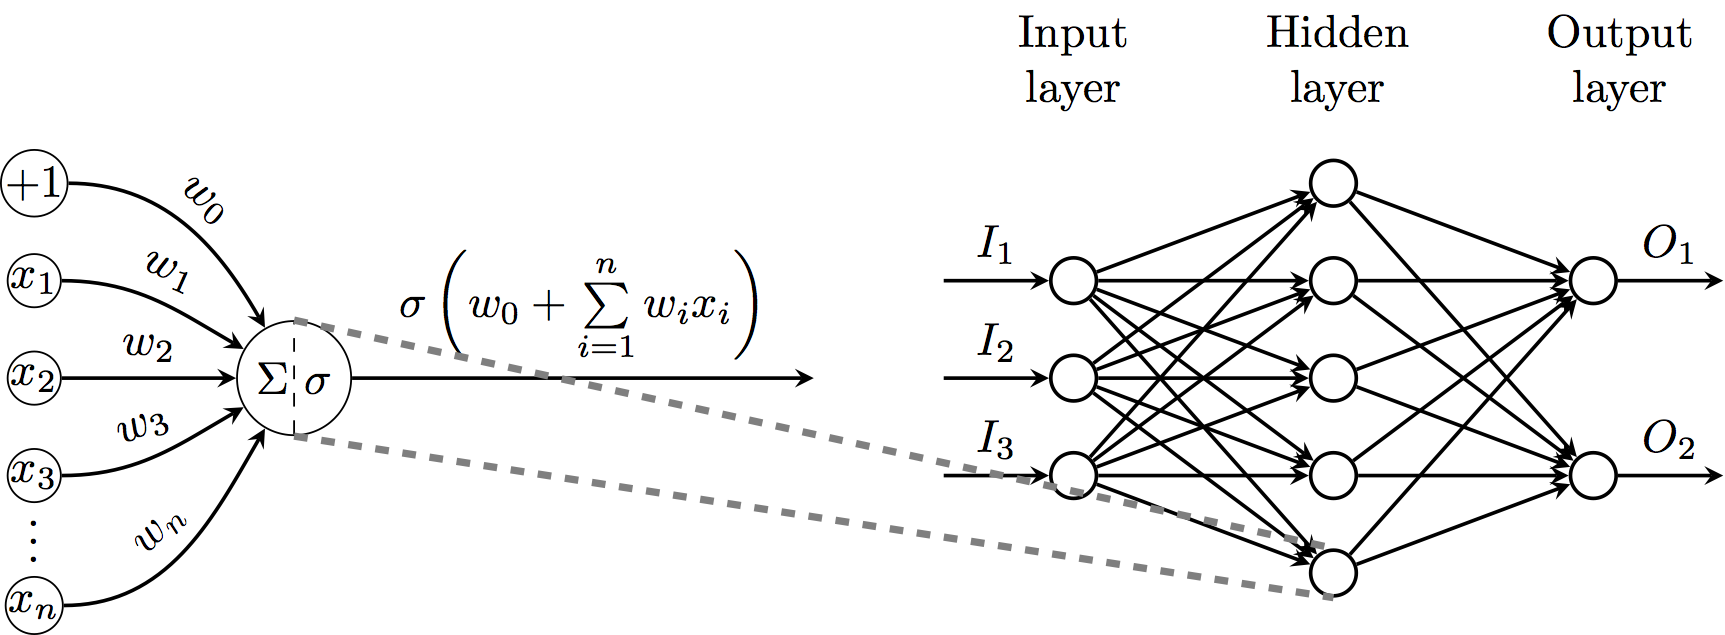
\includegraphics[width=0.95\textwidth]{images/MLP}
	\caption{Multi-Layer-Perceptron (MLP) \cite{Velickovic.2018}}
	\label{fig:mlp}
\end{figure}


Bei diesem Netzwerktyp entspricht der Wert eines Knotens einer linearen Überlagerung $n$ sigmoidaler Funktionen, ausgedrückt durch 

\begin{equation} 
\label{eq:feedforward}
\sigma(w_0 + \sum_{i=1}^{n} w_i x_i)
\end{equation}

Die lineare Überlagerung der Netzwerkgewichte $w_1,w_2,...,w_n$ multipliziert mit den Eingangsgrößen $x_1,x_2,...,x_n$ und verschoben um den Wert $w_0$ wird nochmals durch eine Aktivierungsfunktion transformiert. Mögliche Aktivierungsfunktionen sind die \textit{sigmoidale}-Funktion $\sigma(z) = \frac{1}{1 + e^{-z}}$, die \textit{tangenssigmoidale}-Funktion $\phi(z)=\frac{2}{1 + e^{-2z}}-1$ und die \textit{lineare} Funktion $a(z)=z$. \\ 
Die Auswahl der Aktivierungsfunktion ist hierbei vom konkreten Anwendungsfall abhängig. Das Training bzw. die Parametrisierung des Netzes erfolgt nun in zwei Schritten. Im ersten Schritt findet eine Übergabe der Eingangsgrößen $x_1,x_2,...,x_n$ an das Netz statt. Weiterhin nehmen die Netzwerkgewichte $w$ anfangs zufällige Werte an. Da die Eingangsgrößen und die Netzwerkgewichte bekannt sind, kann jeder Knotenwert nach Gleichung \ref{eq:feedforward} berechnet werden. Die nachfolgenden Knotenwerte der nächsten Schicht lassen sich somit sukzessive als Funktion der vorherigen Schicht berechnen. Auf diese Weise des Vorwärtsrechnens findet eine Transformation der Eingabegrößen $x_1,x_2,...x_n$ in ein Ausgangssignal $\hat{y}$ statt (in Abbildung \ref{fig:mlp} als $O_1$ und $O_2$ bezeichnet). \\
Der zweite Schritt umfasst nun die Adaptierung der Netzwerkgewichte, sodass die vom Netz herausgegebenen Ausgabegrößen $\hat{y}$ mit den gemessenen Ausgabegrößen $y_i$ möglichst übereinstimmen. Dabei ist es zweckmäßig, die Abweichung zwischen diesen Größen in Form der Fehlerfunktion 

\begin{equation}
E(w) = (y_i-N(x|w))^{2}
\end{equation}

zu beschreiben. Die Adaptierung der Netzwerkgewichte beschränkt sich nun darauf, die Fehlerfunktion zu minimieren. Eine der gängigsten Methoden ist die Methode des Gradientenabstieges. Diese gibt als Adaptionsregel für die Netzwerkgewichte 

\begin{equation}
\label{eq:weight_adapt}
\Delta w_i = \epsilon  (-\nabla E_i) = \epsilon * - \dfrac{\partial E}{\partial w}\bigg|_{w_i}
\end{equation}

mit $\epsilon$ als Lernrate bzw. Adaptionsschrittweite vor. Das Ziel besteht darin, für die Fehlerfunktion $E(w)$ die partiellen Ableitungen $\dfrac{\partial E}{\partial w}\bigg|_{w_i}$ zu identifizieren und gleich null zu setzen. Damit würde die Fehlerfunktion $E(w)$ ein lokales Minima erreichen. Dies geschieht durch die lokale Suche nach dem Minimum der Fehlerfunktion $E(w)$ in Richtung des steilsten Abstiegs. Die Richtung des steilsten Abstiegs entspricht dabei dem negativen Gradienten von $E$ nach den Netzwerkgewichten $w_i$.\\ 
Die Adaption findet für jedes vorhandene Datenpaar $((x_1,x_2,...,x_n)|(y_1))$ statt. Durch das Wiederholen des Adaptionsvorgang passt sich das Netz an das zu modellierende Systemverhalten an. \\

Wie bereits erwähnt, bietet sich die Methode des Gradientenabstieges als ein mögliches Verfahren zur Minimierung der Fehlerfunktion an. Es gibt darüber hinaus in der Literatur eine Vielzahl von Verfahren, die sich nach \cite{Sklyarenko.2002} in folgende Kategorien einteilen lassen:

\begin{itemize}
	\item Gradientenverfahren erster Ordnung
	\item Gradientenverfahren zweiter Ordnung
	\item stochastische Optimierungsverfahren
	\item Verfahren der globalen Optimierung
\end{itemize}


\textbf{Backpropagation-Algorithmus}

Den Verfahren der ersten Kategorie ist gemein, dass die Berechnung des Gradienten des Gütefunktionals

\begin{equation}
\nabla E_i = \dfrac{\partial E}{\partial w}\bigg|_{w_i}
\end{equation}

in jeder Iteration problematisch ist, da sich die Gradienten nicht in einem Schritt berechnen lassen. In der Regel kommt für die Lösung dieses Problems der \textit{Backpropagation}-Algorithmus zum Einsatz. Dieser wendet die Kettenregel an, um die Gradienten in mehrere Faktoren, bestehend aus partiellen Ableitungen, zu zerlegen. Auf diese Weise können die partiellen Ableitungen der letzten Schicht, welche in der Regel bekannt sind, benutzt werden können, um die partiellen Ableitungen der vorangehenden Schichten zu bestimmen. Dies ist gleichbedeutend mit dem Belegen der \textit{Jacobi-Matrix}. \\


\begin{figure} 
	\centering
	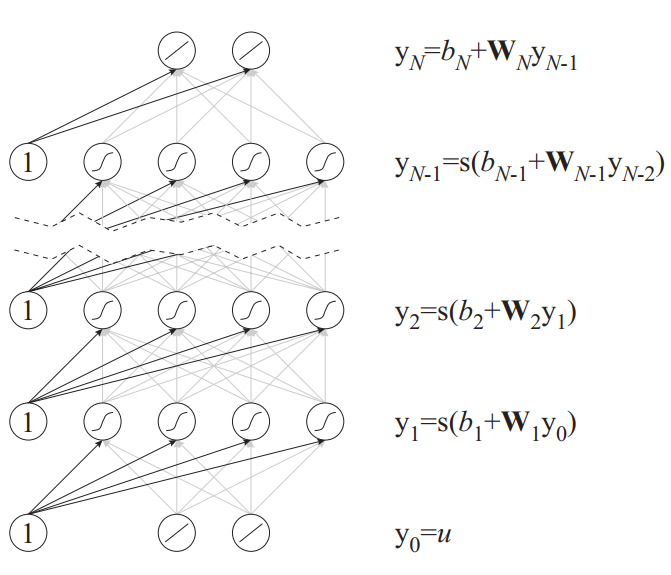
\includegraphics[width=0.65\textwidth]{images/backpropagation2}
	\caption{Multi-Layer-Perceptron \cite{Sturm.2000}}
	\label{fig:backpropagation}
\end{figure}

Die Ermittlung der notwendigen partiellen Ableitungen ergibt sich nach \cite{Sturm.2000} durch folgende Rekursionsformeln \\

\begin{equation}
\begin{aligned}
Y'_{i-1} = Y'_i \cdot S'_i \cdot W_i \\
\dfrac{\partial y_N}{\partial (W_i)_{jk}} = Y'_i \cdot S'_i \cdot \left(\begin{array}{c}
(y_{i-1})_k  \\ ... \\ ... \\ (y_{i-1})_k 
\end{array}\right) \\
\dfrac{\partial y_N}{\partial \vec{b_i}} = Y'_i \cdot S'_i
\end{aligned}
\end{equation}

Dabei enthält die Matrix $Y'_i$ die partiellen Ableitungen der Ausgabegrößen der letzten, also der $N$ten Schicht, nach der $i$ten Schicht. Am Anfang der Rekursion entspricht diese der Einheitsmatrix. Die Matrix $S'_i$ enthält die Ableitungen der Aktivierungsfunktionen der $i$ten Schicht. \cite{Sturm.2000}


Die Ermittlung der partiellen Ableitungen findet also von der letzten bis zur ersten Schicht, also rückwärts, statt. Nach Ermittlung der partiellen Ableitungen aller Schichten, kann die Adaption der Netzwerkgewichte gemäß einer Adaptionsregel, siehe \ref{eq:weight_adapt}, erfolgen. Während des Adaptionsprozesses nimmt der Gesamtfehler ab. Sinkt der Gesamtfehler über alle Netzausgänge $y_1,...,y_m$ unter eine festgelegte Grenze, bricht das Training des Netzes ab. \\


Es bleibt festzuhalten, dass die Anpassungsfähigkeit des Netzes an das nichtlineare Verhalten dynamischer Systeme von folgenden Faktoren abhängt:

\begin{itemize}
	\item Anzahl der Neuronen
	\item Anzahl der Schichten
	\item Wahl des Algorithmus zur Minimierung der Fehlerfunktion
	\item Auswahl der Aktivierungsfunktionen
	\item Repräsentationsfähigkeit der Trainingsdaten
	
\end{itemize}

Die richtige Auslegung der Parameter für das neuronale Netz stellt eine Herausforderung dar. In Abschnitt KAPITEL ist eine ausführliche Diskussion über die Auswahl der Netzparameter, vor allem über den Algorithmus und  die Anzahl der Neuronen, enthalten. \\ 
Das bisher vorgestellte \textit{Feedforward-Netz} ist vor allem dazu geeignet, den statischen Zusammenhang zwischen Eingangs- und Ausgangsgrößen abzubilden. \textit{Feedforward-Netze} sind rein vorwärts gerichtete Netze und definieren sich lediglich über die Eingabegrößen und die Parametrisierung der Gewichte. Somit sind \textit{Feedforward-Netze} zustandsfrei. Davon unterscheiden sich sogenannte \textit{rekurrente Netze}, welche den Einfluss der Zeit zusätzlich berücksichtigen können. 

\subsection{Rekurrente neuronale Netze}

Bei \textit{rekurrenten Netzen} findet - im Gegensatz zu \textit{Feedforward-Netzen} - eine Berücksichtigung des zeitlichen Verlaufs der Eingabe- und Ausgabegrößen statt. Dies wird durch den Einsatz von \textit{rekurrenten Kanten} ermöglicht, welche zwei neuronale Netze in aufeinanderfolgenden Zeitschritten miteinander verbinden, siehe Abbildung \ref{fig:recurrent}.  

\begin{figure} [h]
	\centering
	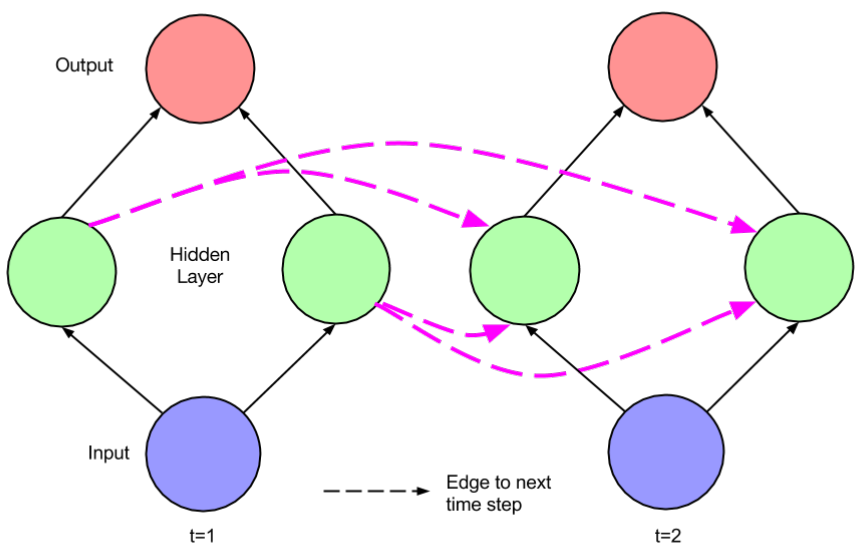
\includegraphics[width=0.75\textwidth]{images/recurrent_net}
	\caption{Rekurrentes Netz \cite{Lipton.5292015}}
	\label{fig:recurrent}
\end{figure}

Die \textit{rekurrenten Kanten} erlauben es, dass die Netzwerkknoten zum Zeitpunkt $t$ nicht nur die Eingabegröße $x(t)$, sondern auch die Ausgabegrößen $h^{(t-1)}$ der verdeckten Knoten des vorherigen Zeitschrittes zum Eingang haben. Der Ausgang des Netzes $\hat{y}^{(t)}$ zum Zeitpunkt $t$ ergibt sich aus dem Ausgang $h^{(t)}$ aller verdeckten Knoten zum Zeitpunkt $t$. Auf diese Weise beeinflusst die Eingangsgröße $x^{(t-1)}$ zum Zeitpunkt $t-1$ die Ausgangsgröße $\hat{y}^{(t)}$ zum Zeitpunkt $t$. Der Ausgang der verdeckten Knoten $h^{(t)}$ zum Zeitpunkt $t$ kann nach \cite{Lipton.5292015} durch 

\begin{equation}
h(t) = \sigma(W^{hx}x^{(t)} + W^{hh}h^{(t-1)} + b_h)
\end{equation}

beschrieben werden. Dabei besteht die Matrix $W^{hx}$ aus den konventionellen Gewichten, welche sich zwischen den Eingabegrößen und den verborgenen Knoten befinden. Die Matrix $W^{hh}$ dagegen besteht aus \textit{rekurrenten Gewichten}, welche sich zwischen den verborgenen Knoten des aktuellen und des vorangegangenen Zeitschrittes befinden. Für die Adaptierung der Netzwerkgewichte kommt bei \textit{rekurrenten Netzen} üblicherweise der \textit{backpropagation-through-time}-Algorithmus zum Einsatz. \cite{Lipton.5292015}












 


 
